\section{Approximate Abstraction on Example Domains}
%Explanation of what abstraction is used
We run experiments on aggregation functions the $\epQ$ abstraction. For each trial our aggregation greedily groups ground states into abstract states that satisfy the $\epQ$ criteria. The order in which ground states are selected and then greedily added is randomized so there is randomization across trials. Every ground state is equally weighted in its abstract state.

%Explanation of what plots done
For each domain we report two quantities as a function of epsilon with \%95 confidence bars. First, we compare the number of states in the abstract \ac{MDP} to different values of $\epsilon$, shown in Figure~\ref{fig:main_empirical_results1}. The smaller this value, the smaller the state space of the $\ac{MDP}$ that the agent must plan over. Second, we report the value under the abstract policy of the initial ground state, shown in Figure~\ref{fig:main_empirical_results2}. 200 Trials are run for each data point.

%Discuss results
\enote{Make sure results discussion is consistent with "the thesis of this work..."}

Our empirical results corroborate our thesis -- that approximate state abstractions can form the basis of learnable and useful state aggregation criteria. In both NChain and Minefield, we observe that despite increasing $\epsilon$ to reduce the number of states which must be planned over, optimal behavior is either fully maintained (NChain) or very nearly maintained (Minefield). Similarly for Taxi and $\epsilon$ between $.02$ and $.025$ we observe a reduction in the number of states in the Abstract MDP while value is fully maintained. After $.025$, increased reduction in state space size comes at a cost of value. Lastly, as $\epsilon$ is increased in the Random domain, there is a smooth reduction in the number of abstract states which must be planned over with a corresponding cost in the value of the derived policy.

Our experimental results also highlight a noteworthy characteristic of approximate state abstraction in goal-based \acp{MDP}. Taxi exhibits relative stability in state space size and behavior for epsilon up to $.02$ until both fall off dramatically. We attribute the sugdden fall off in number of abstract states and value of the derived policy in Taxi to its goal-based nature; once information critical for achieving optimal behavior is lost in the state aggregation, solving the goal -- and so acquiring any reward -- is unattainable. Conversely, in the Random domain, a great deal of near-optimal policies are available to the agent. Thus, even the information for optimal behavior is lost with an increase in $\epsilon$ there are a great deal of near-optimal policies available to the agent which are not lost in the state aggregation.

\enote{Should we regenerate plots for nChain so it has CIs to match other plots?}
% Figure: Epsilon vs. #States and Epsilon vs Abstract Pol. For NChain and Minefield.
\begin{figure}
\label{fig:main_empirical_results1}
\centering

\subfigure[NChain]{
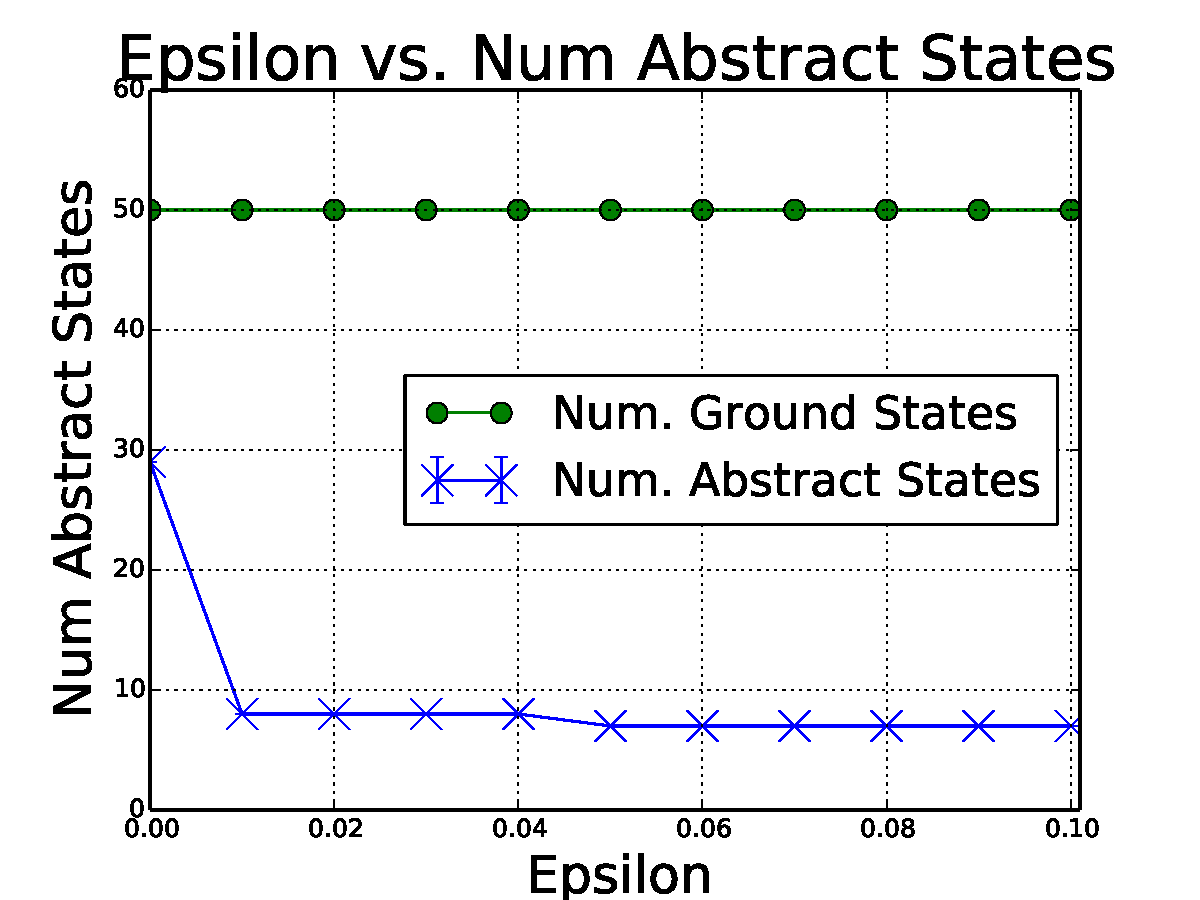
\includegraphics[width=0.46\columnwidth]{figures/nchain_epsilon_vs_num_abstract_states.pdf}
}
\subfigure[NChain]{
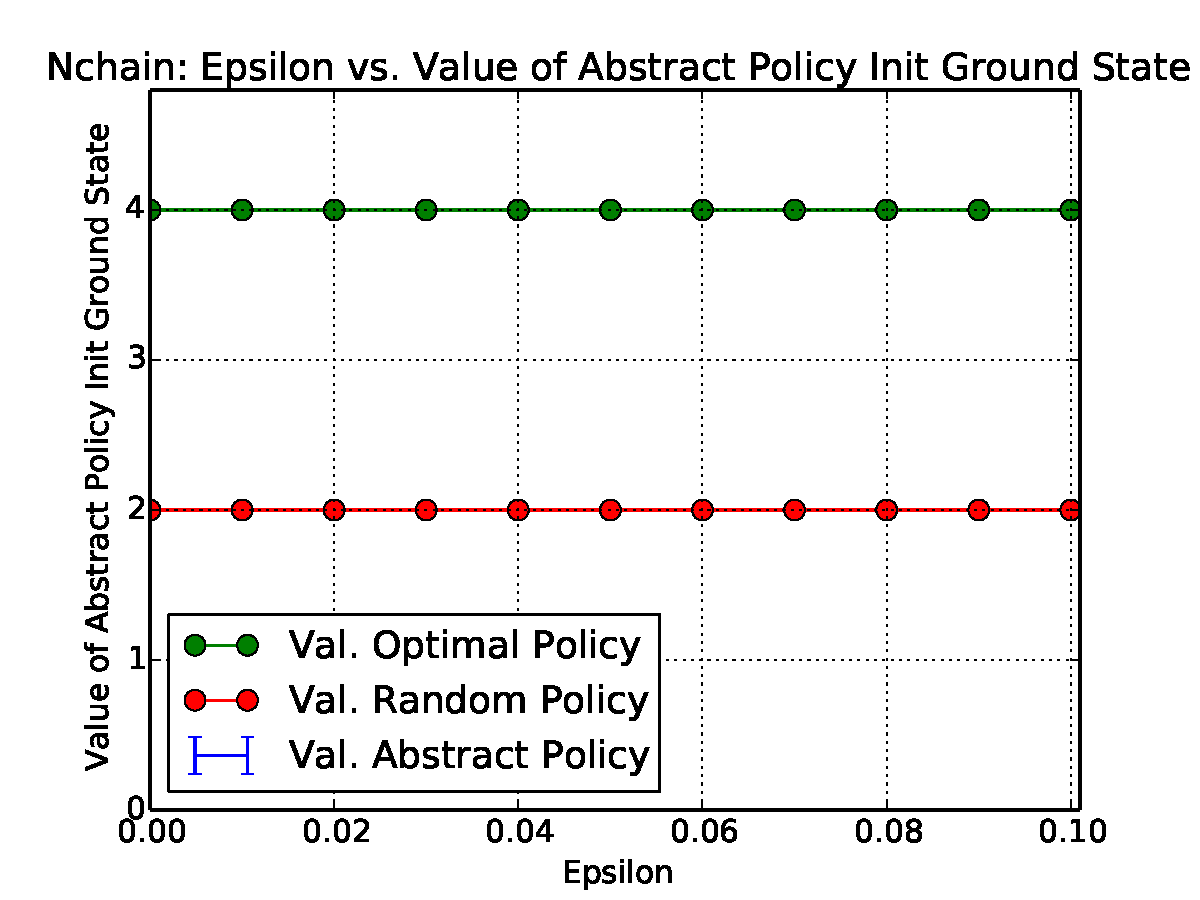
\includegraphics[width=0.46\columnwidth]{figures/nchain_epsilon_vs_value_of_abstract_policy_init_ground_state.pdf}
}

\subfigure[Minefield]{
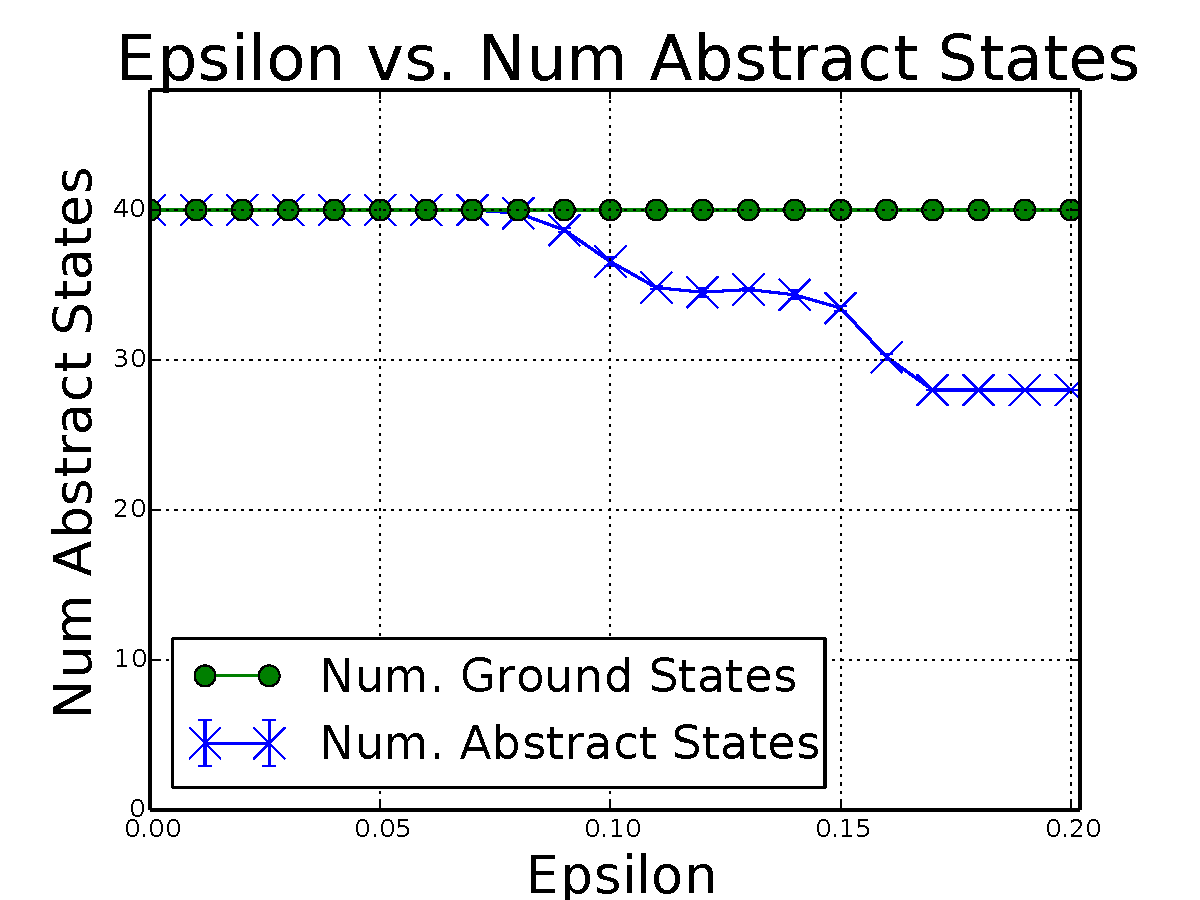
\includegraphics[width=0.46\columnwidth]{figures/minefield_epsilon_vs_num_abstract_states.pdf}
}
\subfigure[Minefield]{
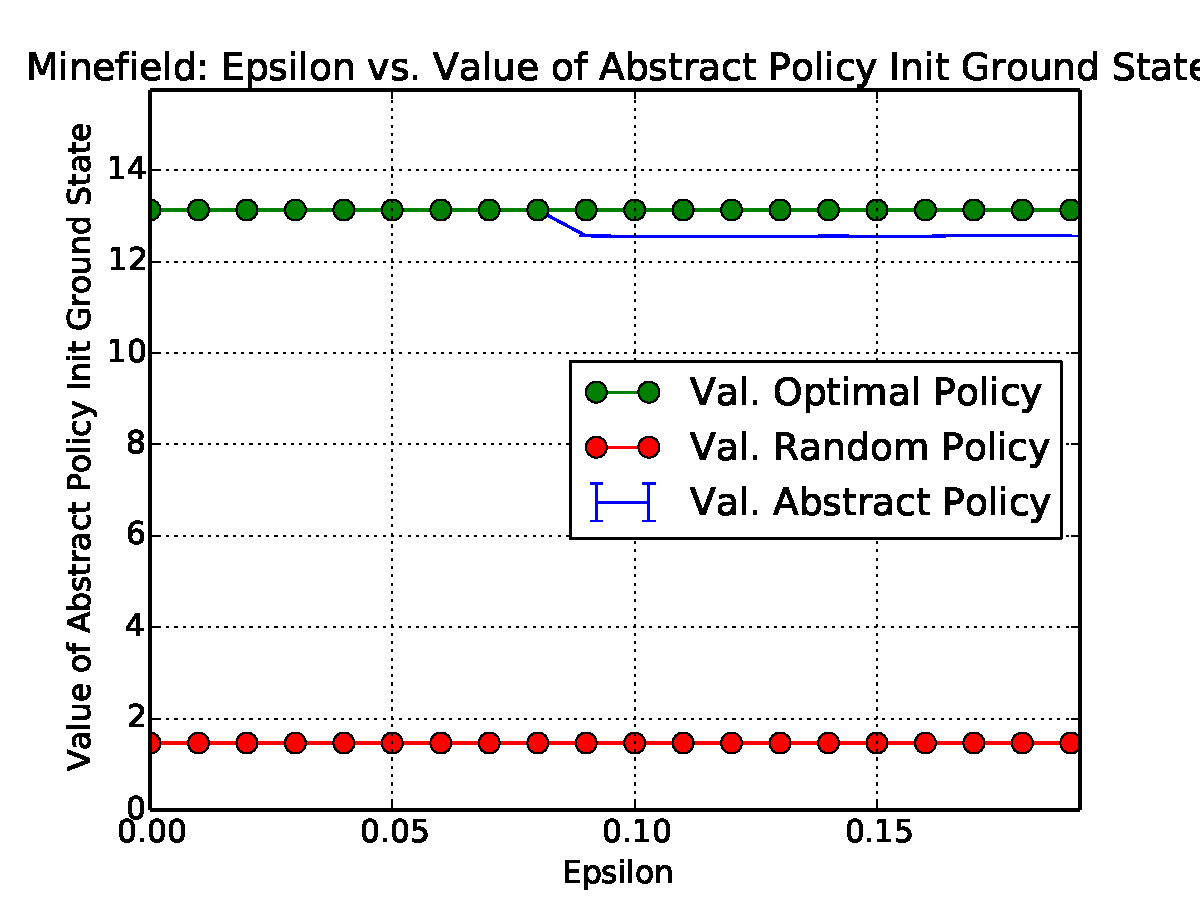
\includegraphics[width=0.46\columnwidth]{figures/minefield_epsilon_vs_value_of_abstract_policy_init_ground_state.pdf}
}

\caption{$\epsilon$ vs. Num States and $\epsilon$ vs. Abstract Policy Value}
\end{figure} 

% Figure: Epsilon vs. #States and Epsilon vs Abstract Pol. For Taxi and Random.
\begin{figure}
\label{fig:main_empirical_results2}
\centering
\subfigure[Taxi]{
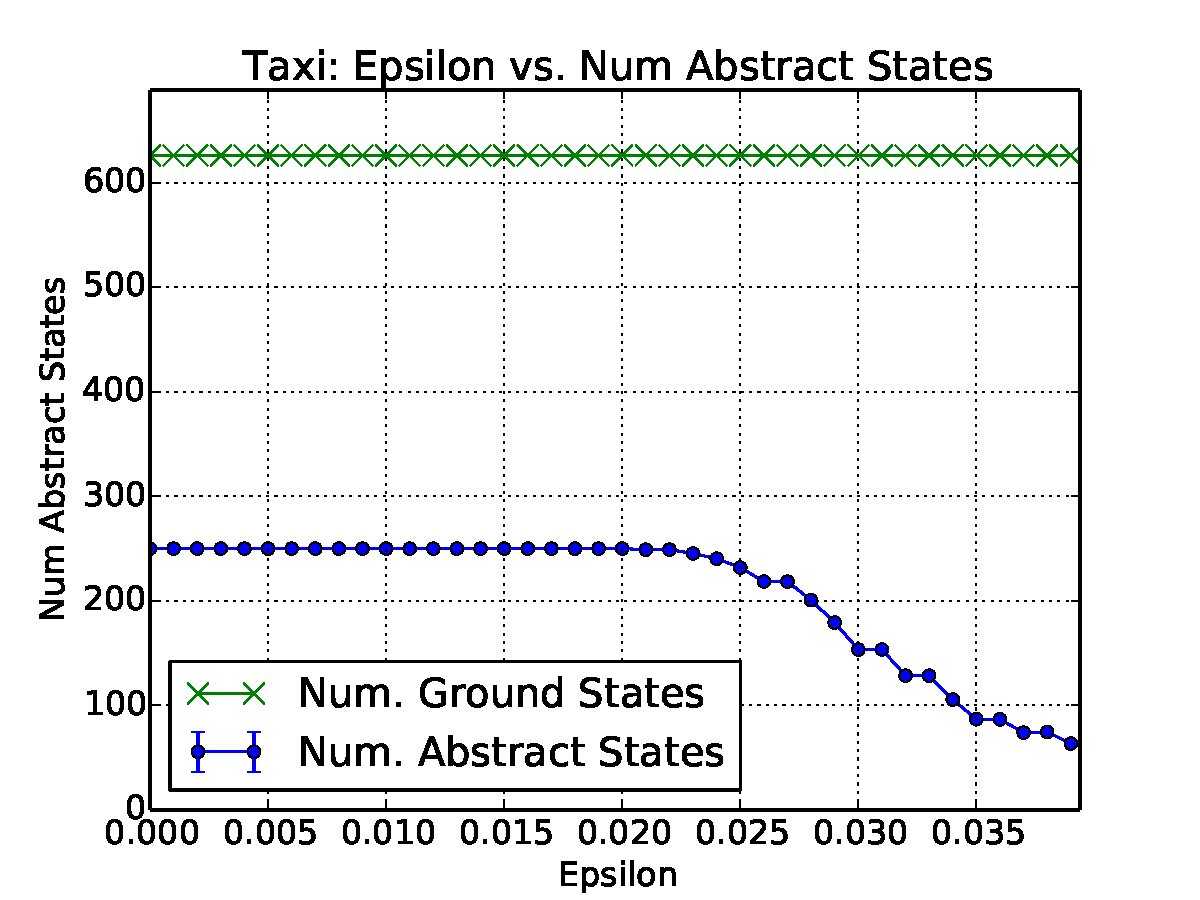
\includegraphics[width=0.46\columnwidth]{figures/taxi_epsilon_vs_num_abstract_states.pdf}
}
\subfigure[Taxi]{
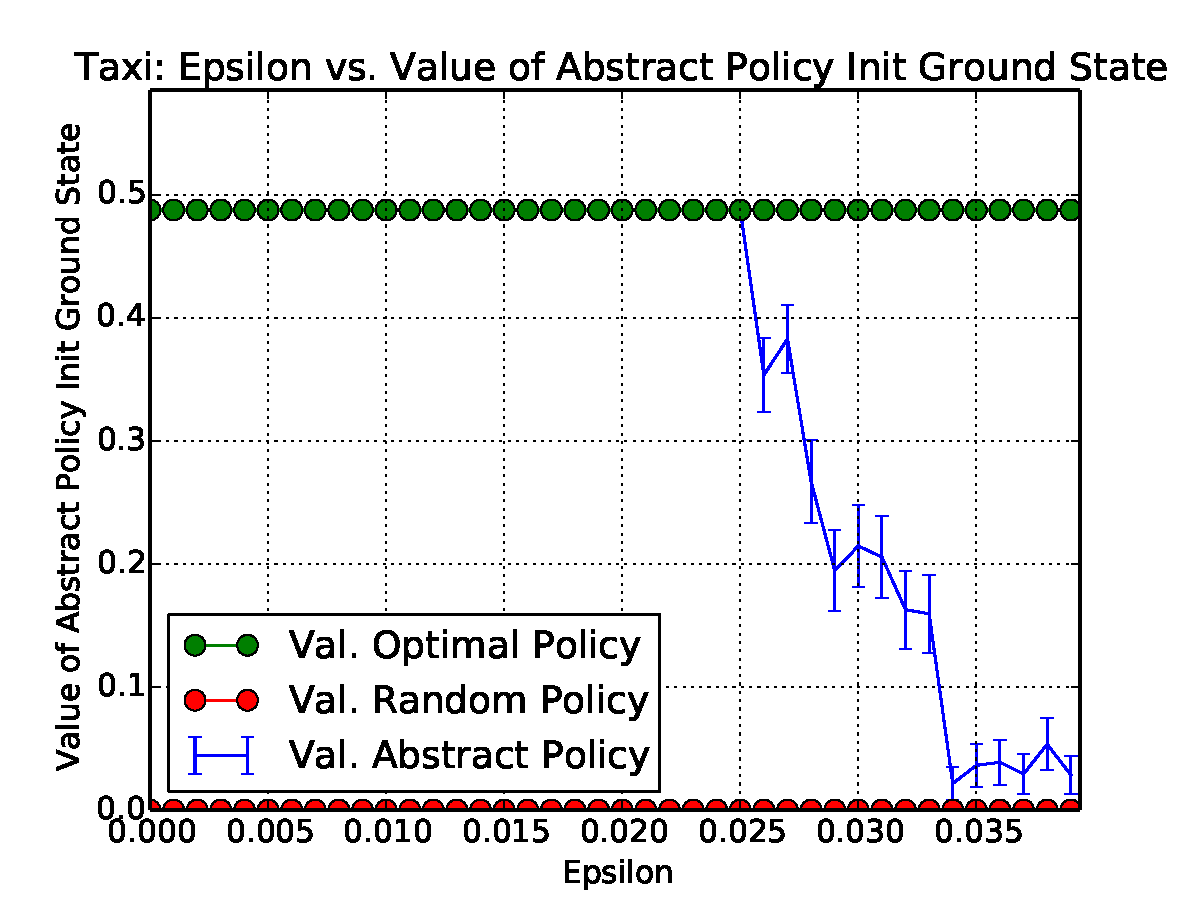
\includegraphics[width=0.46\columnwidth]{figures/taxi_epsilon_vs_value_of_abstract_policy_init_ground_state.pdf}
}

\subfigure[Random]{
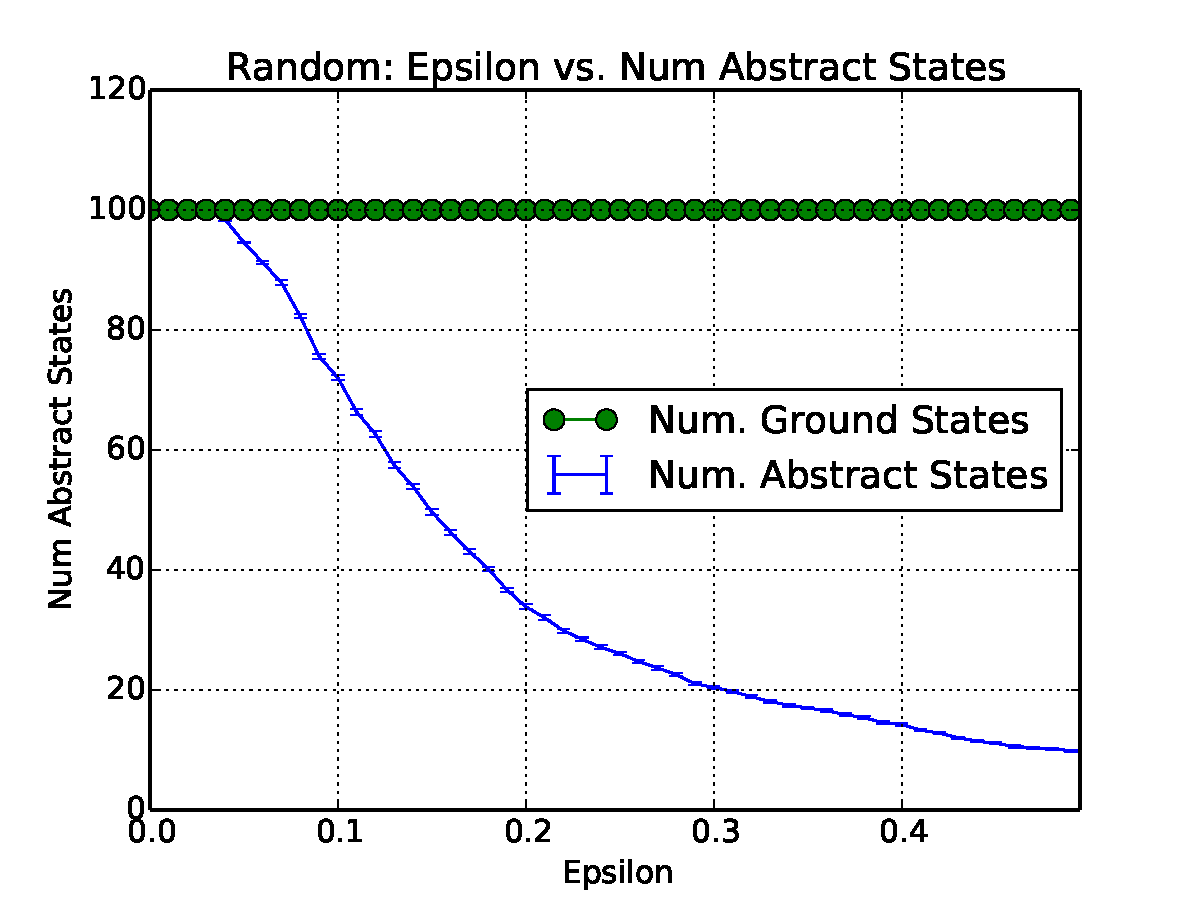
\includegraphics[width=0.46\columnwidth]{figures/random_epsilon_vs_num_abstract_states.pdf}
}
\subfigure[Random]{
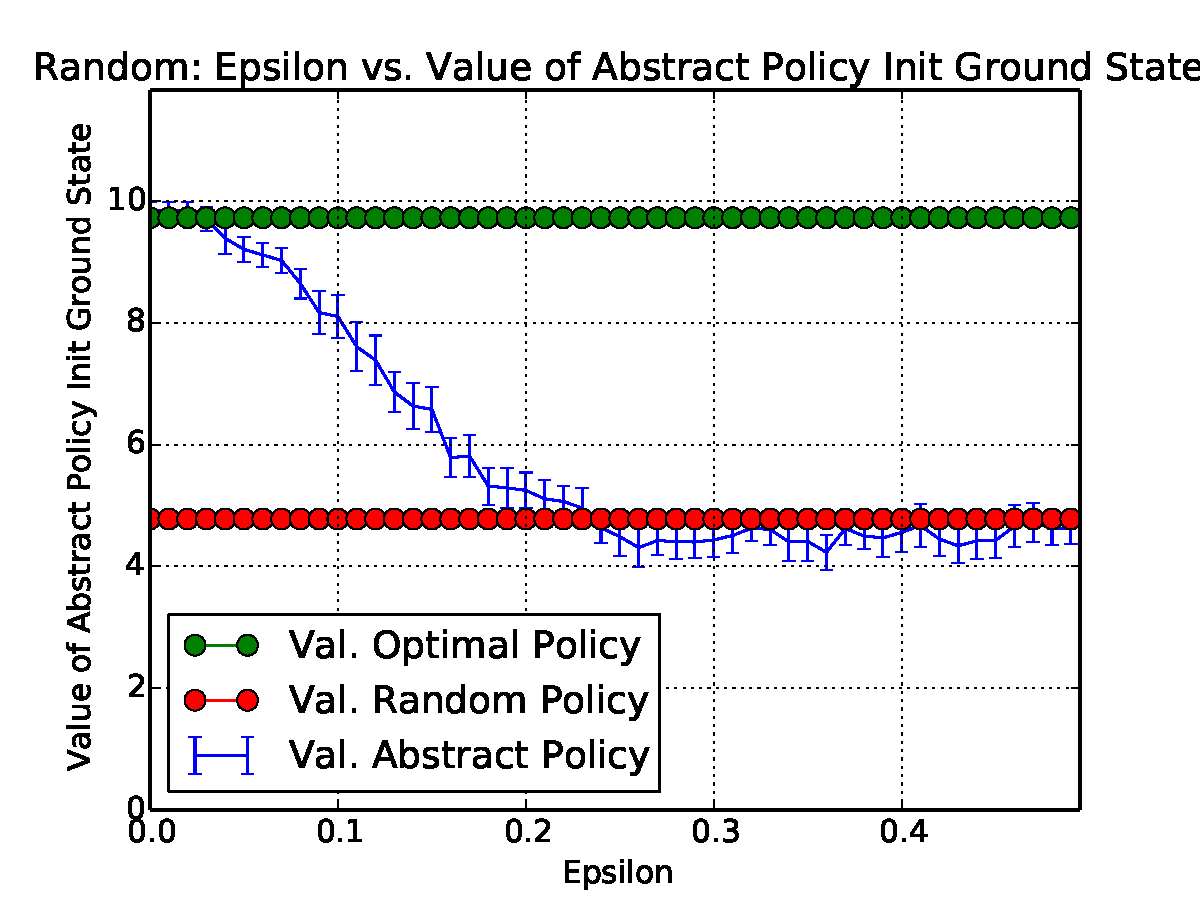
\includegraphics[width=0.46\columnwidth]{figures/random_epsilon_vs_value_of_abstract_policy_init_ground_state.pdf}
}

\caption{$\epsilon$ vs. Num States and $\epsilon$ vs. Abstract Policy Value}
\end{figure} 
